\chapter{Prior and related work}\label{chapter_background_work}
To understand how software trajectory relates to other research, in this chapter I will compare it is u
My research focuses on the techniques which aide in the software process-related knowledge 
discovery from software process artifacts. In this chapter, I review relevant previous work related to my goal.

\section{History of Engineering in software development}
Since the invention of Charles Babbage’s difference engine in 1822, computers (hardware) 
have required a means of instructing them to perform a specific task. This means is known 
as a programming language. By using programming language instructions, 
software develeopers (programmers) write the software that is collections of computer data 
and instructions, which is used by users to accomplish specific tasks. 
The very first software, or more precisely a set of instructions implementing a method for 
calculating a sequence of Bernoulli numbers using Charles Babbage's Analytical Engine, was 
designed by Ada Lovelace in 1942 and predates modern computers. 

As time has progressed, computers have made giant leaps in processing power and become 
general-purpose computing devices. Consequently, the variety of software and 
the complexity of its development has grown ``several orders of magnitude'' \cite{naur_crisis_68}. 
This effectively created a number of organizational problems which dominated development of 
early software systems. Among these, historians are mentioning increasing scale of software projects, 
excessive ambition, difficulties in estimating project cost and length, inadequate documentation, 
skimping on design and testing \cite{mahoney_roots_1990} \cite{citeulike:12748733} 
\cite{citeulike:833903}.

All these problems were acknowledged at the NATO Conference on Software Engineering, held in Garmisch,
Germany in 1968. It worth noting, that before the actual conference, as was pointed by the 
conference proceedings editors, the engineering paradigm was chosen without actual plan of actions - 
\textit{``the phrase ``software engineering'' was deliberately chosen as being provocative, in implying 
the need for software manufacture to be [based] on the types of theoretical foundations and practical 
disciplines[,] that are traditional in the established branches of engineering''} \cite{citeulike:12787786}.
At the conference, it was recognized, that the increasing complexity of programming 
work had overwhelmed the technical and managerial ability of software teams: software was shipped late,
over budget, worked inefficiently, and was unreliable. Later, while working on the proceedings, the term 
``software crisis'' was coined by the editors in order to describe the desperate state of 
software development and its increasing complexity \cite{naur_crisis_68}.

The ``software engineering'' idea happened to be provocative enough to shape the minds of researchers 
and practitioners. At large, it was accepted that the software can be successfully ``manufactured'' 
through ``engineering'' - i.e. with the application of a systematic, disciplined, quantifiable approach 
to the design, development, operation, and maintenance. 

Using this paradigm, researchers and practitioners designed a number of software development processes 
providing detailed guidelines on how to reach the goal - deliver a software - efficiently and in time. 
These processes were declared as the means for software development improvements in terms of quality, 
speed, and execution cost over existing practices. 
They were studied extensively within academic settings and in industry. Most efficient processes were 
further standardized, shaping the best practices of contemporary software development \cite{citeulike:9962021}. 
These can be found in numerous studies and described at length in academic and industrial literature. 
Too numerous to name, they can be categorized by the level of their application:
\begin{itemize}
 \item global organizational standards, like CMMI, ISO 9000, and SPICE. 
 \item large industrial software models, such as Waterfall, Spiral, Cleanroom, etc.
 \item smaller scale, flexible methodologies: FDD, TDD, Pair Programming, etc.
 \item general guidelines and principles aiming to improve the software process flow, 
such as ``build before commit'' and others.
 \item and finally, the processes for improving existing processes of software development 
on the organizational, team, and personal levels: TSP, PSP, Six Sigma, etc.
\end{itemize}
While some of these are products of a ``technology transfer'' - resulted by direct copying or by an 
application of existing engineering principles to software development process (like Waterfall model), 
some, and in particular agile methodologies, considered to be particular to software-engineering. 

Currently,  there are numerous software process, models, methodologies, and coding conventions exist 
in Software Engineering. This amount of well-grounded and documented knowledge creates an impression,
that the area of software development is thoroughly explored, and that there always exists a deterministic 
choice for a model and a processes for any given software project, leaving almost no doubts in 
its faith - it will be completed according to the specification, in time, and under the budget.

However, it is far from being true - software projects do fail at the very high rate and many challenges 
exist at the level of software processes. Software projects continue to run over the budget and do not 
meet the schedule. Some of the seemingly proper executed projects caused property 
damage \cite{citeulike:11044022}, and a few projects caused loss of life \cite{citeulike:712058}. 
The ``Chaos Report'' from the Standish Group concluded, that only ``35\% of software projects in 2006 
can be categorized as successful - meaning they were completed on time, on budget and met 
user requirements'' \cite{chaos2006}, which clearly manifested that it is somewhat illusory statement 
that we are capable to understand and to control software processes using engineering paradigm.

In recent decades, gradually, researchers and practitioners alike recognized, that a direct application 
of classical engineering - that excludes a ``human component'' by governing software processes 
in a top-down fashion might be erroneous. 
Also, it was recognized that over many years, continuous formalization of the field and 
excessive attention to software process metrics may malformed not only the software development 
practices landscape, but education and the professional code of conduct. 
This recognition forced some of the professional associations to review their licensing policies 
\cite{citeulike:11045517} and even some educators to change their opinions \cite{citeulike:5203446}. 

\section{Alternative software processes}
In parallel with industrial engineering-like software processes, another phenomena, the Free/Libre Open 
Source Software (FLOSS) development arose and proven its efficiency and effectiveness.
The FLOSS processes are significantly different from typical SE process on many levels:
\begin{itemize}
 \item First of all, FLOSS processes are highly geographically distributed, which significantly contradicts 
 to developers collocation usually assumed by the most of the SE processes. 
 \item Secondly, open-source processes do not explicitly define timeline, developers roles, and 
 the process itself. Typically, the project flow is rarely governed and does not require any sort of 
 documented software process. Most of FLOSS projects accept for review and embed source code from anyone.
 \item Finally, FLOSS delivers software free of charge, promoting its reuse, modification, and redistribution.
 However, mostly due to this, the maintenance and the support are rarely provided.
\end{itemize}

Nevertheless, despite to the apparent lack of the control over the software processes in FLOSS projects, they 
has proven their ability to deliver large in size software systems of high quality for the fraction of cost 
of similar industrial projects.

Most of the success is contributed to the motivation of open source developers.

Lately, third approach to software development emerged - software craftsmanship emerged 
\cite{citeulike:11058561}, \cite{citeulike:11058554}. The followers of this methodology 
are not only focused on the delivering ``well crafted'' software and continuously adding value,
but on the apprenticeship - on forming communities and engaging more people in software development.
While recommendation exists \cite{citeulike:11058784}, little known about the research 
in software craftsmanship and apprenticeship processes.

All this continues to engage thoughts and fuels the search not just for the exact definition 
of software development, but deep, fundamental for efficient processes resolving. 
Is software development an engineering discipline? Is it a craft \cite{citeulike:5203446}? 
Or is it an art \cite{citeulike:11045694}?


. Among others, 
Free/Libre/Open-Source Software development model (FLOSS) and the Software Craftsmanship 
approaches gained a significant credibility in the community \cite{citeulike:3729379}. 
While the former \textit{holistic} software process paradigm emphasizes loosely-organized 
collaboration, high degree of modularity, frequent releases, and effectively removes the boundary 
between developers and users, the latter, human-centric approach, is built upon the roles of highly 
motivated skilled individuals \cite{citeulike:262020} \cite{citeulike:2759198}. 

Answers to these questions would require extensive interdisciplinary studies to be made, 
but what is obviously clear, is that formal software development process, as an engineering 
is a creative, human activity. 
Whether software is coded 
by team where its members have a variety of skills and experience, or by a single individual,
they all driven by their believes and motivations. While usually developers agree on the use of 
particular technologies, development tools, and a development process with imposed timeline and 
a budget, the software process is - as many other human activities - highly creative and mostly 
non-recurring. Thus, the choice of methodology, technology, or tools provides only a marginal 
effect on this human-based and human-driven process. While this effect can be measured through 
the common approach by using a control environment factoring out human component, the most of 
the difference, which lies in human creativity, motivation and productivity is unknown and yet, 
mostly immeasurable.

\section{Process discovery}\label{process.discovery} 
Process is a general term describing a phenomenon unfolding in time and has a variety of meaning depending
on the field. While in this thesis I focus on a particular kind - software processes, moreover, on the particular process 
building block - recurrent behaviors, in this section I outline few general conceps and previous research work that 
was applied to software processes.

\subsection{Stochastic process}
In probability theory a stochastic (or a random) process denotes a collection of random variables which typically used
to represent the evolution of some random value or a non-deterministic system in time. The specificity of a stochastic 
process is that while its initial condition is known, it can evolve in infinitely many directions. 
In the simple case of discrete time, a stochastic process amounts to a sequence of random variables usually known as 
a stochastic time series. 
The examples of stochastic time series include signals such as speech, audio and video, medical data such as a 
patient's EKG, blood pressure or temperature, stock market and exchange rate fluctuations, and random movement 
such as Brownian motion or random walks.

The common approach to stochastic processes treats them as functions of one or several deterministic arguments whose 
values are random variables that taken from parametrized probability distributions. For example the growth of a software 
project size can be modeled by its relationship with time and effort as was shown by numerous research work 
\cite{citeulike:330266} \cite{citeulike:12849755} \cite{citeulike:12849753} \cite{citeulike:328047} \cite{citeulike:12849771}
which suggests that the evolution of various software metrics can be modeled with Double Pareto distribution.

While stochastic process is useful for predicting of what likely to be observed, they usually are too low level to be used for
a software process modeling. For example a variety of development events such as maintenance, correction, new function,
and enhancement may cause change in a number of source code files and lines, but in order to discover these events 
from the metrics changes an additional mapping procedure, such as coding performed by human experts or classification 
with automated techiques is required. Once mapping is applied, a number of tools and techniques usually called ``business 
intelligence tools'' can be applied to these collections of events.

Although process mining in the business domain is a well-established field with much software developed up to date 
(ERP, WFM and other systems), ``Business Process Intelligence'' (BPI) tools usually do not perform process discovery and 
typically offer relatively simple domain-oriented analyses that depend upon a correct a-priori process model 
\cite{citeulike:3718014} \cite{citeulike:5044991}. 
This fact restricts off-shelf application of business domain process mining techniques to software engineering, where 
processes are usually performed concurrently by many agents, are more complex and typically have a higher level of noise. 
Taking this fact in account, I will review only the approaches to stochastic process mining for which applicability to software 
process mining was expressed. 

In particular I review four approaches in the rest of this section: 
\begin{itemize}
 \item the work by Cook \& Wolf in that discuss an event-based framework for process discovery based on grammar 
  inference and finite state machines. 
  The authors directly applied their framework to Software Configuration Management (SCM) logs demonstrating satisfactory 
  results \cite{citeulike:328044}.
 \item the work by Van der Aalst et al. where they demonstrate the applicability of Transition Systems and labeled Petri nets 
  to process discovery in general \cite{citeulike:3718014} and the subsequent work by van der Aalst and Rubin 
  that discusses software process mining \cite{citeulike:1885717}.
 \item the approach by Jensen \& Scacchi \cite{citeulike:5043664} that describes a framework built upon an universal generic 
  meta-model and specific to the observed processes models which are iteratively built and revised during case studies. 
  The particular value of this work is in the demonstration of the importance of the correct mapping between process artifacts 
  and process entities as well as a demonstration of iterative process revision that emphasizes the importance of pre-existing 
  domain knowledge in the effective pruning of the search space.
\item the recent work by Hindle et al. \cite{citeulike:9114115} \cite{citeulike:9007622} that shows the possibilty of software 
  process evidence discovery from software process artifacts.
\end{itemize}

Notice, that all reviewed approaches require a mapping to be provided. In addition all reviewed approaches have difficulties 
dealing with concurrency, which, in turn, is inevitable in the software process usually performed by many agents. 
Much successive work has been done extending reviewed approaches to the concurrent processes. 
%Among others, Weijters \& van der Aalst in \cite{citeulike:5128101} propose heuristics to handle concurrency and noise issues, 
%while van der Aalst et al. in \cite{citeulike:5128110} discuss a genetic programming application. 

\subsection{Process discovery through Grammar Inference} \label{grammar}
One of the pioneering process discovery techniques was developed by Cook \& Wolf in \cite{citeulike:328044}. The authors 
developed a generic techniques intended to discover process models from event streams. The authors did not really intend to 
generate a complete model, but rather to generate sub-models that express the most frequent patterns in the event stream.
They designed a framework which collects process data from ongoing software process or from history logs, and generates a 
set of recurring patterns of behavior characterizing observed process. In their work they extended two methods of 
\textit{grammar inference} from previous work: purely statistical (neural network based \textit{RNet}) and purely algorithmic 
(\textit{KTail}) as well as developed their own Markovian method (\textit{Markov}). 

\textit{Process discovery}, in the author's opinion, resembles the process of \textit{grammar inference}, which can be defined 
as the process of inferring a language grammar from the given set (sample) of sentences in this language. 
In the demonstrated approach, words of the language are atomic events of the dynamic process, whether sentences built from 
such words, are describing the behavior of a process. 
Consequently, the inferred grammar of that language is the formal model of the process. Cook \& Wolf expressed such grammars 
as Finite State Machines (FSMs) and implemented a software tool for the mining of the software process. 
This tool was successfully tested in an industrial case study.

\begin{figure}[tbp]
   \centering
   \includegraphics[width=140mm]{inference.eps}
   \caption{Process discovery through the grammar inference: panel a) a sample event stream (simple process involving three 
   types of events: Edit, Review, and Checkin); and FNA results obtained by applying three methods of process discovery from 
   Cook \& Wolf \cite{citeulike:328044}.}
   \label{fig:inference}
\end{figure}

The first method extended by the authors, the neural-network based grammar inference, RNet algorithm, defines a recurrent 
neural network architecture which is trained by the sequences of events. After training, this neural net is able to characterize a 
current system state by looking on past behavior. The authors extract the FSM from the trained neural network by presenting 
different strings to it and extracting the hidden neurons activity through observations. Due to the nature of Neural Net, closely 
related activation patterns are clustered into the same state; therefore, by noting the current pattern, the input token, and the 
next activation pattern, transitions are recorded and compiled into the inferred FSM.

The second method investigated, is a purely algorithmic KTail method, which was taken from the work of 
Biermann \& Feldman \cite{citeulike:5120603}. The idea is that a current state is defined by what future behaviors can occur 
from it. The \textit{future} is defined as the set of next $k$ tokens. By looking at a window of successor events, the KTail 
algorithm can build the equivalence classes that compose the process model. The authors extensively modified the original 
KTail algorithm improving the folding in the mined model making to make it more robust to noise.

The Markov based method developed by the authors is based on both algorithmic and statistical approaches. 
It takes to account past and future system behavior in order to guess the current system state. Assuming that a finite number 
of states can define the process, and that the probability of the next state is based only on the current state (Markov property), 
the authors built a $n^{th}$-order Markov model using the first and second order probabilities. Once built, the transition 
probability table corresponding to the Markov model is converted into FSM which is in turn reduced based on the user-specified 
cut-off threshold for probabilities.

The authors implemented all three of these algorithms in a software tool called \textsc{DaGama} as a plugin for larger software
system called Balboa \cite{citeulike:5120757}. By performing benchmarking, Cook \& Wolf found that the Markov algorithm was 
superior to the two others. RNet was found to be the worst of the three algorithms. 

Overall, while having some issues with the complexity of produced output and noise handling, the authors proved applicability 
of implemented algorithms to real-world process data by demonstrating an abstraction of the actual process executions and 
capturing important properties of the process behavior. The major backdraw of the approach, as stated by the authors, 
lies in the inability of the FSMs to model concurrency of processes which limits its applicability to the software development process.
Later, they addressed this limitation \cite{citeulike:5128143}.


\subsection{Incremental Workflow Mining with Petri Nets}
Another set of findings relevant to my research approach was developed by Rubin
et al. \cite{citeulike:1885717} and van der Aalst et al.
\cite{citeulike:3718014} and is called \textit{incremental workflow mining}. The
authors not only designed sophisticated algorithms but built a software system
using a business process mining framework called ProM by van Dongen et al.
\cite{citeulike:5043673} which synthesizes a Petri Net corresponding to the
observed process. The system was tested on SCM logs and while the process
artifacts retrieved from the SCM system are rather high-level, the approach
discussed is very promising for the modeling of software processes from the
low-level product and process data.

\begin{figure}[tbp]
   \centering
   \includegraphics[height=65mm]{petri.eps}
   \caption{Illustration of the ``Generation and Synthesis Approach'' from
\cite{citeulike:5043673}: a) Transition System with regions shown; b),c) Petri
Nets synthesized from the Transition System.}
   \label{fig:petri}
\end{figure}

Within the incremental workflow mining framework, the input data from the SCM
audit trail information is mapped to the event chain which corresponds to the
software process artifacts. The authors call this process \textit{abstraction on
the log level} which is implemented as a set of filters which not only
aggregates basic events into single high-level entities but also removes data
irrelevant to the mining process (noise). 

The event chain constructed through the abstraction is then treated with the
\textit{Generate} part of the \textit{``Generate and Synthesis''}
\cite{citeulike:3718014} algorithm in order to generate a \textit{Transition
System} which represents an ordered series of events. This algorithm looks at
the history (prefix) and the future (suffix) sequences of events related to the
current one in order to discover transitions.  When applied to the abstracted
log information, the algorithm generates a rather large Transition System graph
where edges connect to abstracted events. This transition system is then
successively simplified by using various reduction strategies such as ``Kill
Loops'', ``Extend'', ``Merge by Output'' and others; it is possible to combine
these reduction strategies in order to achieve a greater simplification.

At the last step of the incremental workflow mining approach, Transition Systems
are used to \textit{Synthesize} labeled Petri nets (where different transition
can refer to the same event) with the help of \textit{``regions theory''}
\cite{citeulike:5128170}. As with the Transition System generation, the authors
investigate many different strategies of Petri nets synthesis, showing
significant variability in the results achieved. (see Figure \ref{fig:petri}).

The significant contribution of this research is in the generality of the
method. It was shown that by tuning the ``Generate'' and ``Synthesize'' phases
it is possible to tailor the algorithm to a wide variety of processes. In
particular, as mentioned before, Rubin et al. successfully applied this
framework to the SCM logs analysis.

\subsection{Reference model for Open Source Software Processes Discovery}
Jensen \& Scacchi in \cite{citeulike:5043664} take a somewhat different approach from the previously discussed research efforts. The authors are follow a top-down approach and do not try to build a software process model from available process artifacts. Instead, they try to develop a software process \textit{reference model} by iteratively refining mapping between observed artifacts and the model entities. 

The proposed software process \textit{reference model} is a layer which provides a mapping from the underlying recognized software process artifacts into a higher level software-process meta-model by Mi \& Sacchi \cite{citeulike:5128872}. The iterative revision of the reference model vocabulary of mapped terms (Figure \ref{fig:refterm}) is performed through case studies. During such a study, the observed process artifacts such as SCM logs, defect reports and others are queried with terms from the reference model pulling correlated artifacts which are revised and curated by the process expert and lead to the further revisions of the terms taxonomy on the next iteration.

\begin{figure}[tbp]
   \centering
   \includegraphics[height=35mm]{refterm.eps}
   \caption{Example of the reference model mapping from \cite{citeulike:5043664}.}
   \label{fig:refterm}
\end{figure}

In the relation to my research, I am envisioning the application of such iterative ``meta-model driven approach'' for characterization of the discovered recurrent patterns with unknown generative phenomena. The creation of the low-level recurrent patterns taxonomy through successive mapping into the meta-model assures from a ``nonsense patterns'' discovery.

\section{Mining software repositories}
However, in these and other research work based on mining of software process artifacts it was shown, 
that while public availability of artifacts is minimizing observability and privacy issues, the nature 
of these artifacts creates a number of other challenges, which limit the possible scope of the research 
and significantly elevate the complexity of the process discovery:
\begin{itemize}
\item First of all, the artifacts are created by developers and users not in order to enable the research,
but merely to support software development activities. Thus, the process-related information content of these
artifacts is questionable.
\item Secondly, the majority of these artifacts (change records, defect reports, assigned tasks, etc) 
typically represent a snapshot of the software project state rather than reflect any of performed actions, 
thus it might be simply impossible to infer any of completed software development events \cite{citeulike:1296888}.
This fact effectively renders obsolete a majority of previously developed event-based process discovery tools.
\item Thirdly, developers and users not only create and submit to repositories artifacts on their own volition,
but most of the change management system (such as Git, Subversion, and Gerrit) offer an asynchronous workflow, 
where the locally created artifacts might never be committed \cite{citeulike:2280690} \cite{citeulike:9037939}. 
Therefore, artifacts are displaced in time and it is often impossible to know exactly when their content was created.
\item Finally, the high volume of produced artifacts and their dimensionality demands for automated, high throughput 
techniques robust to the noise \cite{citeulike:12550438}, \cite{citeulike:7853299}, \cite{citeulike:4534888}.
\end{itemize}

While many behaviors are simply not observable through artifacts because they are never recorded
and do not leave any quantifiable evidence behind, for example phone-calls, face-to-face meetings, and 
private communications. 

\section{Knowledge discovery in time series}
